\documentclass{exercise}

\setcounter{exercise}{6}
\newcommand{\topics}{The Halting Problem, Complexity Theory}
\newcommand{\distdate}{07.12.2020}
\newcommand{\duedate}{18.12.2020}

\title{\line(1,0){415}\\
  Foundations of Computing II\\
  \Large Assignment \theexercise\ -- Solutions\\[1em]
  \large{\topics}\\
  \line(1,0){415}}

\lefttitle{Universit\"at Z\"urich\\Institut f\"ur Informatik\\[1em]
  \textsl{Student Name:}\\
  \textsl{Student Number:}}
\righttitle{Autumn 2020\\Sven Seuken\\Dennis Komm} 

\begin{document}

\maketitle

\begin{center}
  Distributed: \distdate\ -- Due Date: \duedate\\[1em]
  Upload your solutions to the OLAT system.\\[3em]
\end{center}

\task{The Halting Problem}

In the lecture, we reduced the universal language $L_{\text{U}}$ to the halting
problem $L_{\text{H}}$.  Using a similar approach, now reduce $L_{\text{H}}$
to $L_{\text{U}}$.

\begin{solution}
  This time, we suppose that we are given a TM $U^*$ that decides $L_{\text{U}}$, and we construct
  a TM $H^*$ that decides $L_{\text{H}}$ using $U^*$; by definition, both TMs always halt.
  The following figure is essentially the same as for the reduction from $L_{\text{U}}$ to
  $L_{\text{H}}$.

  \begin{center}
    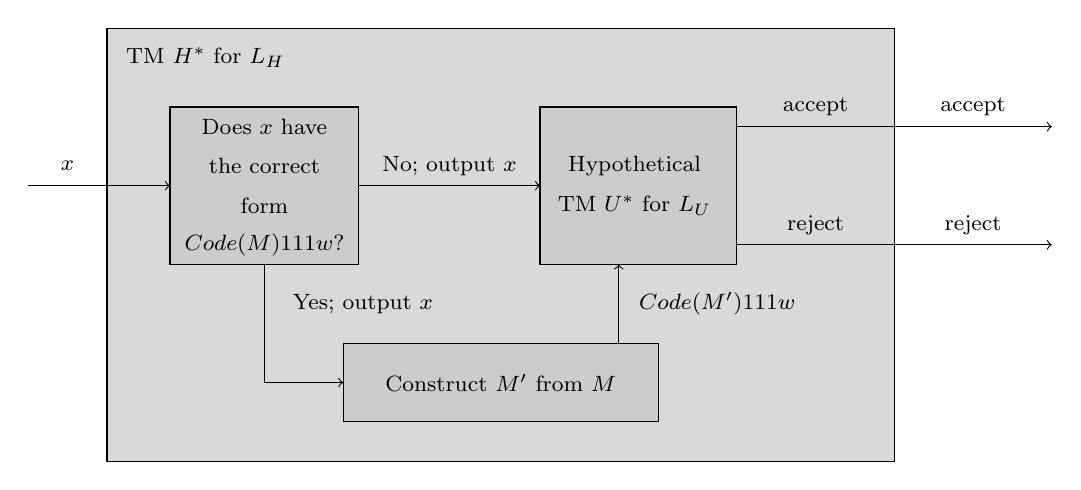
\begin{tikzpicture}[font=\footnotesize]
      \draw[fill=gray!30] (0,-2) rectangle (10,3.5);
      \draw[fill=gray!40] (5.5,2.5) rectangle (8,0.5);
      \draw[fill=gray!40] (0.8,2.5) rectangle (3.2,0.5);
      \draw[fill=gray!40] (3,-0.5) rectangle (7,-1.5);
      \node at (1.25,3.125) {TM $H^*$ for $L_{\text{H}}$};
      \node at (6.7,1.75) {Hypothetical};
      \node at (6.7,1.25) {TM $U^*$ for $L_{\text{U}}$};
      \node at (2,2.25) {Does $x$ have};
      \node at (2,1.75) {the correct};
      \node at (2,1.25) {form};
      \node at (2,0.75) {$\text{Code}(M)111w$?};
      \node at (5,-1.0) {Construct $M'$ from $M$};
      \node at (-0.5,1.75) {$x$};
      \node at (4.35,1.75) {No; output $x$};
      \node at (3.25,0) {Yes; output $x$};
      \node at (7.75,0) {$\text{Code}(M')111w$};
      \draw[->] (-1,1.5) -- (0.8,1.5);
      \draw[->] (3.2,1.5) -- (5.5,1.5);
      \draw[->] (8,0.75) -- (12,0.75);
      \draw[->] (8,2.25) -- (12,2.25);
      \draw[->] (2,0.5) -- (2,-1.0) -- (3,-1.0);
      \draw[->] (6.5,-0.5) -- (6.5,0.5);
      \node at (9,2.5) {accept};
      \node at (9,1) {reject};
      \node at (11,2.5) {accept};
      \node at (11,1) {reject};
    \end{tikzpicture}
  \end{center}

  The reduction is indeed very similar to the original one given in the
  lecture.  Only the roles of $U^*$ and $H^*$ have been switched and the TM $M'$ is
  constructed from the given TM $M$ in a different way, as described in what follows.

  This time, we want to know whether $M$ halts, but we can only decide (using $U^*$)
  whether $M'$ accepts.
  The idea is to once more consider all the states in which $M$ may get stuck.
  In this reduction, there is no new state added, but these ``missing'' transitions are
  added such that they end in an accepting state.  We then have the
  equivalence
  \[ M \text{ halts on } w \iff M' \text{ accepts } w\;. \]

  Therefore, the answer of $U^*$ as to whether $\text{Code}(M')111w$ is in $L_{\text{U}}$ can be
  taken as the correct answer as to whether $\text{Code}(M)111w$ is in $L_{\text{H}}$.

  It follows that, if $L_{\text{U}}$ were recursive, $L_{\text{H}}$ would also
  be recursive.
\end{solution}


\task{Closure Properties of Languages in \boldmath$\mathcal{P}$\unboldmath}

Show that the languages in $\mathcal{P}$ are closed under the following
operations.  Argue on an intuitive, but exact level.

\subtask \textbf{Union}, \ie, if $L_1,L_2\in\mathcal{P}$, then $L_1\cup L_2\in\mathcal{P}$,

  \begin{solution}
    Let $L_1$ and $L_2$ be any two languages such that $L_1,L_2\in\mathcal{P}$.
    Now we want to prove that also $L_1\cup L_2\in\mathcal{P}$.  Let $w$ be any
    word for which we want to decide in polynomial time whether it is in
    $L_1\cup L_2$. In other words, we want to decide whether $w\in L_1$ or
    $w\in L_2$.

    By definition, there is a TM $M_1$ that decides whether $w$ is in $L_1$,
    and there is a TM $M_2$ that decides whether $w$ is in $L_2$. 

    A TM $M$ for $L_1\cup L_2$ first uses $M_1$ to decide whether $w\in L_1$.

    \begin{itemize}
      \item If $w\in L_1$, $M$ accepts.
      \item If $w\notin L_1$, $M$ uses $M_2$ to decide whether $w\in L_2$.
      \item If $w\in L_2$, $M$ accepts.
      \item Otherwise $M$ rejects (\ie, halts in a non-accepting state).
    \end{itemize}

    Since both $M_1$ and $M_2$ run in polynomial time, $M$ also runs in
    polynomial time; thus, $L_1\cup L_2$ is in $\mathcal{P}$ as a direct
    consequence of the existence of $M$.
  \end{solution}

\subtask \textbf{Intersection}, \ie, if $L_1,L_2\in\mathcal{P}$, then $L_1\cap L_2\in\mathcal{P}$,

  \begin{solution}
    A TM $M$ for $L_1\cap L_2$ works similar to that described in the solution
    of a).  The only difference is that this TM only accepts if $M_1$ and $M_2$
    both accept the input $w$; otherwise it rejects.
  \end{solution}

\subtask \textbf{Complement}, \ie, if $L\in\mathcal{P}$, then $\overline{L}\in\mathcal{P}$.

  \begin{solution}
    Let $M$ be a TM for $L$ that runs in polynomial time.  A TM $\overline{M}$
    for $\overline{L}$ simulates $M$ on the given input.
    
    \begin{itemize}    
      \item If $M$ accepts, $\overline{M}$ rejects.
      \item If $M$ rejects, $\overline{M}$ accepts.
    \end{itemize}    

    Clearly, $\overline{M}$ runs in polynomial time and thus $\overline{L}\in\mathcal{P}$.
  \end{solution}

\nosubtask

\textit{Hint:} In the lecture, we have seen that the regular languages are closed
  under quite a few operations.  This was done by starting with the DFAs for
  the given languages and then modifying them.  Use an analogous approach to
  answer the above questions.

\task{Polynomial-Time Reductions}

In complexity theory, SAT plays the same role for us as $L_{\text{diag}}$ in
computability theory.  To show that a problem is $\mathcal{NP}$-hard, we can
reduce SAT to it.

In the lecture, we have introduced the satisfiability problem (SAT and $3$SAT),
the independent set problem IND-SET, the clique problem CLIQUE, and the vertex
cover problem VC; then we proved $\text{SAT}\le_{\textsf{p}}3\text{SAT}$,
$3\text{SAT}\le_{\textsf{p}}\text{IND-SET}$, $\text{IND-SET}\le_{\textsf{p}}\text{CLIQUE}$,
and $\text{IND-SET}\le_{\textsf{p}}\text{VC}$, which implies that all of them
are $\mathcal{NP}$-hard.

Here, we introduce three other problems which we prove to be
$\mathcal{NP}$-hard by polynomial-time reductions.

\subtask The set cover problem SC is defined as follows.  An input is triple
  $(X,\mathcal{S},k)$ with 
  \begin{itemize}
    \item $X=\{1,2,\dots,n\}$ for some $n\in\nat^+$,
    \item $\mathcal{S}=\{S_1,S_2,\dots,S_m\}$ with $S_i\subseteq X$ for some $m\in\nat^+$ and $X=\bigcup_{j=1}^m S_j$, and
    \item $k\in\nat^+$.
  \end{itemize}
	The question is whether there is a set cover of $X$ of size (at most) $k$,
	\ie, a selection of (at most) $k$ sets from $\mathcal{S}$ such that every
	element from $X$ is contained in at least one of the selected sets, \ie,
	whether there exist $S_{i_1},S_{i_2},\dots,S_{i_k}$ with
	$i_j\in\{1,2,\dots,m\}$ and
  \[ X=\bigcup_{j=1}^k S_{i_j}\;. \]
 
  Formally,
  \[ \text{SC} = \{(X,\mathcal{S},k) \mid X \text{ has a set cover from } \mathcal{S} \text{ of size } k\}\;. \]
  
  As an example, the instance $(X_1,\mathcal{S}_1,3)$ with $X_1=\{1,2,3,4,5,6,7,8\}$ and
  \[ \mathcal{S}_1 = \big\{ \{1,3\}, \{1,2,5\}, \{1,4\}, \{3,4,6\}, \{5,6,8\}, \{5,7,8\} \big\} \]
  is a ``yes'' instance, because there is a set cover
  \[ \{1,2,5\} \cup \{3,4,6\}\cup \{5,7,8\} = X_1 \]
  of size $3$.  Conversely, the instance $(X_2,\mathcal{S}_2,4)$ with $X_2=\{1,2,3,4,5,6,7,8,9\}$
  and
  \[ \mathcal{S}_2 = \big\{\{1,2\}, \{2,3\}, \{2,4,6\}, \{4,5,6\}, \{6,7\}, \{7,9\}, \{8,9\} \big\}. \]
  is a ``no'' instance (as we can cover at most eight elements with three sets from $\mathcal{S}_2$).

  Reduce VC to SC.

  \begin{solution}
    Consider an instance $(G,k)$ of VC with $G=(V,E)$.  We construct an instance
    $(X,\mathcal{S},k)$ of SC by mapping the edges to the elements of $X$ since
    they need to be covered, and we map each vertex to the set of its incident
    edges, because the vertices are used to cover the edges.

    More formally, let $V=\{v_1,v_2,\dots,v_m\}$ and $E=\{e_1,e_2,\dots,e_n\}$,
    where the edges are ordered in an arbitrary but fixed way.
    We set $X=\{1,2,\dots,n\}$; hence, each element of $X$ corresponds to one edge
    of $G$. Then we set $\mathcal{S}=\{S_1,S_2,\dots,S_m\}$ with
    \[ S_i = \{j\in\{1,2,\dots,n\} \mid \text{the edge } e_j \text{ is incident to } v_i \}\; .\]

    As an example of this reduction, consider the instance $(G,2)$ of VC where $G=(V,E)$
    with $V=\{v_1,v_2,v_3,v_4,v_5,v_6\}$ and
    \[ E = \big\{ \{v_1,v_3\}, \{v_2,v_4\}, \{v_3,v_5\}, \{v_3,v_6\}, \{v_4,v_6\} \big\}\;, \]
    which is shown in the following figure.
  
    \begin{center} 
      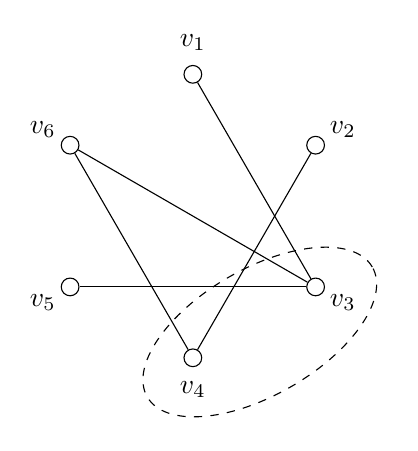
\begin{tikzpicture}[every node/.style={shape=circle,draw=black,fill=none,minimum size=2.25mm,inner sep=0pt},]
        \newcommand{\radius}{1.8cm}
        \newcommand{\labelradius}{2.2cm}
        \foreach \i in {0,...,5}{
          \pgfmathtruncatemacro{\indexcircle}{\i+1};
          \node (\i) at ({90- 360/6*\i}:\radius) {};
          \node[draw=none] at ({90- 360/6 * \i}:\labelradius) {$v_{\indexcircle}$};
        }
        \draw (0) edge (2);
        \draw (1) edge (3);
        \draw (2) edge (4);
        \draw (2) edge (5);
        \draw (3) edge (5);
        \draw[dashed,rotate=30] (0,-1.7) ellipse (1.65cm and 0.8cm);
      \end{tikzpicture}
    \end{center} 

    For some fixed order, let $\{v_1,v_3\}$ be the first edge $e_1$, let $\{v_2,v_4\}$ be
		the second edge $e_2$ etc.

    This is a ``yes'' instance, since there is a vertex cover $\{v_3,v_4\}$ of size $2$,
    which is circled with a dashed line.

    Applying our reduction, we obtain a set cover instance $(X,\mathcal{S},2)$ as
    follows.  We set $X=\{1,2,3,4,5\}$ since there are five edges that need
    to be covered, and $\mathcal{S}=\{S_1,S_2,S_3,S_4,S_5,S_6\}$ with
    \[ S_1 = \{1\},\ S_2=\{2\},\ S_3=\{1,3,4\},\ S_4=\{2,5\},\ S_5=\{3\},\ \text{ and } S_6=\{4,5\}\;, \]
    where, \eg, $S_3$ corresponds to the vertex $v_3$, which is incident to the
    edges $e_1$, $e_3$, and $e_4$.
    We observe that the vertex cover $\{v_3,v_4\}$ translates to a set cover
    $\{S_3,S_4\}$ covering $X$ and vice versa.

    In general, every vertex cover of size $k$ covers all edges of $G$;
    the corresponding set cover then covers $X$ and vice versa, which
    follows directly from the construction.
    
    In conclusion, we have
    \[ G \text{ contains a vertex cover of size } k \iff X \text{ has a set cover from } \mathcal{S} \text{ of size } k\;, \]
    and the construction can clearly be done in polynomial time.
  \end{solution}

\subtask A dominating set in a graph $G=(V,E)$ is a set $D$ of vertices such
  that every vertex from $V$ is either in $D$ or has an edge to at least
  one vertex in $D$; we call such a vertex ``dominated.\!''

  An instance of the dominating set problem DOM-SET is a pair $(G,k)$ where $G$
  is a graph and the question is whether $G$ contains a dominating set of size
  $k\in\nat^+$ (or smaller).

  Formally,
  \[ \text{DOM-SET} = \{(G,k) \mid G \text{ contains a dominating set of size } k\} \;. \]

  Reduce SC to DOM-SET.

  \begin{solution}
    Let $(X,\mathcal{S},k)$ be an instance of SC with $X=\{1,2,\dots,n\}$,
    $\mathcal{S}=\{S_1,S_2,\dots,S_m\}$, and $k\in\nat^+$.  We construct an
    instance $(G,k)$ with $G=(V,E)$ of DOM-SET as follows.  The vertices of $G$ can
    be partitioned into two disjoint sets
    \[ V_X = \{x_1,x_2,\dots,x_n\} \quad \text{ and } \quad V_{\mathcal{S}}=\{s_1,s_2,\dots,s_m\} \;, \]
    where $V_X$ corresponds to $X$ and $V_{\mathcal{S}}$ corresponds to
    $\mathcal{S}$.
    
    The edges $E$ of $G$ are defined as follows.  First, there is an
    edge between any two vertices from $V_{\mathcal{S}}$; \ie, $V_{\mathcal{S}}$
    is a clique.  Second, 
    \[ \{x_i,s_j\}\in E \iff i\in S_j\;; \]
    \ie, there is an edge between a vertex from $V_X$ and a vertex from $V_{\mathcal{S}}$
		if and only if the element $i\in X$ is covered by $S_j\in\mathcal{S}$.

    As an example, consider the instance $(X,\mathcal{S},2)$ of SC with
    $X=\{1,2,3,4,5,6\}$ and
    \[ \mathcal{S} = \big\{\{1,3,4\}, \{2,4\}, \{2,5,6\}, \{4,6\}, \{5,6\} \big\}\;, \]
    where $S_1=\{1,3,4\}$, $S_2=\{2,4\}$ etc.

    We construct the instance $(G,2)$ of DOM-SET with $G=(V,E)$ where
    \[ V = \{x_1,x_2,x_3,x_4,x_5,x_6\} \cup \{s_1,s_2,s_3,s_4,s_5\} \]
    and
    \begin{align*}
      E = \big\{ {}& \{s_1,x_1\}, \{s_1,x_3\}, \{s_1,x_4\}, \\
                   & \{s_2,x_2\}, \{s_2,x_4\},\\
                   & \{s_3,x_2\}, \{s_3,x_5\}, \{s_3,x_6\}\\
                   & \{s_4,x_4\}, \{s_4,x_6\},\\
                   & \{s_5,x_5\}, \{s_5,x_6\}\big\}\;,
    \end{align*}
    which is shown in the following figure.
    \begin{center}
      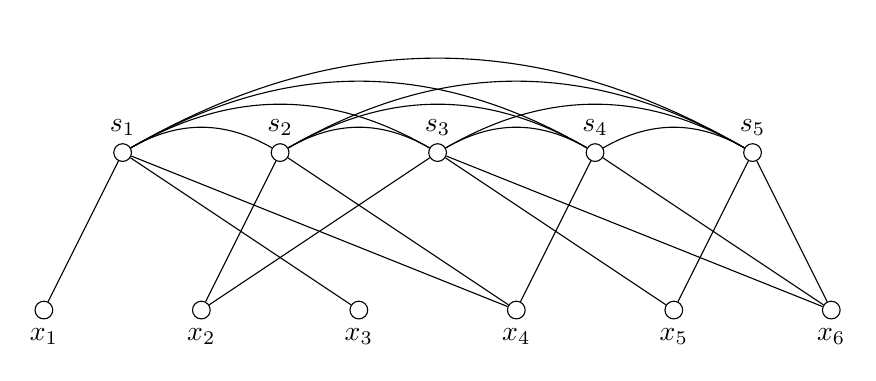
\begin{tikzpicture}[every node/.style={shape=circle,draw=black,minimum size=2.25mm,inner sep=0pt}]
        \newcommand{\filled}{none}
        \foreach \i in {1,...,5} {
          \ifthenelse{\equal{\i}{1} \OR \equal{\i}{3}}{\renewcommand{\filled}{black}}{}
          \node[fill=\filled,label={$s_{\i}$}] (s\i) at (2*\i,2)  {};
        }
        \foreach \i in {1,...,6} {
          \node[label=below:{$x_{\i}$}] (x\i) at (2*\i-1,0) {};
        }
        \newcommand{\bended}{bend left}
        \foreach \k in {4,...,1} {
          \foreach \i in {1,...,\k} {
            \ifthenelse{\equal{\k}{4}}{\renewcommand{\bended}{}}{}
            \pgfmathtruncatemacro{\j}{\i+(5-\k)};
            \draw (s\i) edge[\bended] (s\j)  {};
          }
        }
        \draw (s1) edge (x1);
        \draw (s1) edge (x3);
        \draw (s1) edge (x4);
        \draw (s2) edge (x2);
        \draw (s2) edge (x4);
        \draw (s3) edge (x2);
        \draw (s3) edge (x5);
        \draw (s3) edge (x6);
        \draw (s4) edge (x4);
        \draw (s4) edge (x6);
        \draw (s5) edge (x5);
        \draw (s5) edge (x6);
      \end{tikzpicture}
    \end{center}

    The SC instance $(X,\mathcal{S},2)$ is a ``yes'' instance since there is a set cover
    $\{S_1,S_3\}$ of size $2$, which translates to a dominating set $\{x_1,x_3\}$ in $G$,
    which is marked by filled vertices.

    In general, consider any set cover of $X$ of size $k$.  Selecting
    the corresponding vertices from $V_{\mathcal{S}}$ results in a dominating set
    of $G$ of size $k$, because
    \begin{itemize}
      \item trivially, as soon as one vertex from $V_{\mathcal{S}}$ is selected, all vertices
        from $V_{\mathcal{S}}$ are dominated, because $V_{\mathcal{S}}$ is a clique;
      \item all vertices from $V_X$ are dominated by at least one of the selected vertices
        from $V_{\mathcal{S}}$, because all elements from $X$ are contained in at least one
        of the selected sets from $\mathcal{S}$.
    \end{itemize}

    Conversely, consider any dominating set $D$ of $G$ of size $k$.  If all vertices
    from $D$ are from $V_{\mathcal{S}}$, the corresponding selection of sets from $\mathcal{S}$
    results in a set cover of $X$ of size $k$.
    
    On the other hand, for each vertex $x$ from $D$ that is not from $V_{\mathcal{S}}$ but
    from $V_{X}$, we can choose an arbitrary adjacent vertex from $V_{\mathcal{S}}$ instead.
    This does not increase the size of $D$.  Clearly, $x$ will still be dominated afterwards,
    the other vertices of $V_X$ will still covered, and the vertices from
    $V_{\mathcal{S}}$ will also definitely be covered since $D$ now contains a vertex from
		$V_{\mathcal{S}}$.

    It follows that
    \[ X \text{ has a set cover from } \mathcal{S} \text{ of size } k \iff G \text{ contains a dom.\ set of size } k \;, \]
    and again it is easy to see that the construction can be done in polynomial time.
  \end{solution}

\subtask A half-clique is a clique that contains exactly half of
  the vertices of a given graph.  An instance of HALF-CLIQUE is a graph $G$
  and the question is whether $G$ contains a half-clique.
  
  Formally, 
  \[ \text{HALF-CLIQUE} = \{G\mid G \text{ contains a half-clique} \}\;. \]
  
  Note that, if $G$ contains a clique with more than half of its vertices,
  it also contains a half-clique.

  Reduce CLIQUE to HALF-CLIQUE.

  \begin{solution}
    Let $(G,k)$ be an instance of CLIQUE, and let $n$ denote the number of
    vertices of the graph $G$.  We distinguish two cases.

    \textit{Case 1.} Suppose that $k$ is at least $n/2$, \ie, the given
    CLIQUE instance asks about the existence of a clique that contains more
    than half of the vertices of $G$.  In this case, we add $k'$ vertices to
    obtain a new graph $G'$ with $n'=n+k'$ vertices such that $(n+k')/2=k$
    (this means $k'=2k-n$ vertices are added).  The newly added vertices are all
    isolated, \ie, they are not connected to any other vertex and are
    therefore not part of any clique.

    The idea is shown in the following figure.
    \begin{center}
      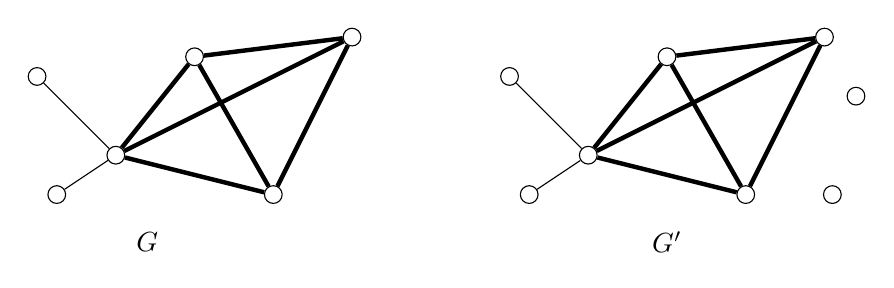
\begin{tikzpicture}[every node/.style={shape=circle,draw=black,fill=none,minimum size=2.25mm,inner sep=0pt}]
        \node (0) at (0,0) {};
        \node (1) at (2,-0.5) {};
        \node (2) at (3,1.5) {};
        \node (3) at (1,1.25) {};
        \node (4) at (-1,1) {};
        \node (5) at (-0.75,-0.5) {};
        \draw (0) edge[ultra thick] (1);
        \draw (0) edge[ultra thick] (2);
        \draw (0) edge[ultra thick] (3);
        \draw (1) edge[ultra thick] (2);
        \draw (1) edge[ultra thick] (3);
        \draw (2) edge[ultra thick] (3);
        \draw (0) edge (4);
        \draw (0) edge (5);
        \node[draw=none] at (0.4,-1.1) {$G$};
        \begin{scope}[xshift=6cm]
          \node (0) at (0,0) {};
          \node (1) at (2,-0.5) {};
          \node (2) at (3,1.5) {};
          \node (3) at (1,1.25) {};
          \node (4) at (-1,1) {};
          \node (5) at (-0.75,-0.5) {};
          \node (6) at (3.1,-0.5) {};
          \node (7) at (3.4,0.75) {};
          \draw (0) edge[ultra thick] (1);
          \draw (0) edge[ultra thick] (2);
          \draw (0) edge[ultra thick] (3);
          \draw (1) edge[ultra thick] (2);
          \draw (1) edge[ultra thick] (3);
          \draw (2) edge[ultra thick] (3);
          \draw (0) edge (4);
          \draw (0) edge (5);
          \node[draw=none] at (1,-1.1) {$G'$};
        \end{scope}
      \end{tikzpicture}
    \end{center}

    $G$ has $6$ vertices and contains a clique of size $4$, which is marked by
    thick edges.  $G'$ has $8$ vertices and a clique of $4=8/2$ vertices (that
    is, a half-clique).
  
    In general, we have the equivalence
    \[ G \text{ contains a clique of size } k \iff G'\text{ contains a clique of size } k\;, \]
    where $k$ is exactly half of the vertices in $G'$.

    \textit{Case 2.} Suppose that $k$ is less than $n/2$.  Then  we again add
    $k'$ vertices to $G$ to obtain a new graph $G'$.  This time, however, $k'$
    is such that $k'+k$ equals exactly half of the vertices from $G'$, \ie,
    $k+k'=(n+k')/2$ (which means that $k'=n-2k$ vertices are added).  All new
    vertices are connected to each other such that they form a clique of size
    $k'$ in $G'$.  Moreover, every such new vertex is connected to \emph{all}
    other vertices from $G$.
    
    The idea is shown in the following figure.
    \begin{center}
      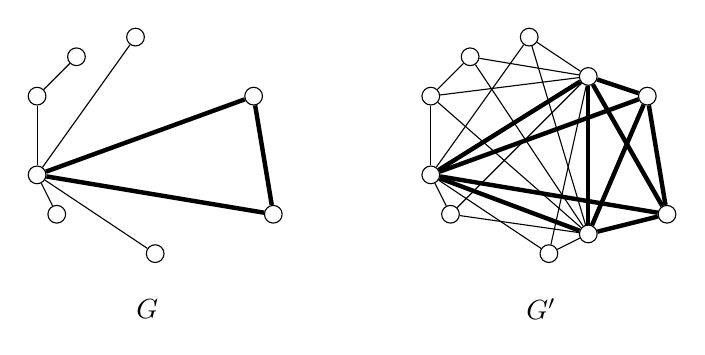
\begin{tikzpicture}[every node/.style={shape=circle,draw=black,fill=none,minimum size=2.25mm,inner sep=0pt},]
        \node (0) at (-1,0) {};
        \node (1) at (2,-0.5) {};
        \node (2) at (1.75,1) {};
        \node (3) at (0.25,1.75) {};
        \node (4) at (-1,1) {};
        \node (5) at (-0.75,-0.5) {};
        \node (6) at (-0.5,1.5) {};
        \node (7) at (0.5,-1) {};
        \draw (0) edge[ultra thick] (1);
        \draw (0) edge[ultra thick] (2);
        \draw (1) edge[ultra thick] (2);
        \draw (0) edge (3);
        \draw (0) edge (4);
        \draw (0) edge (5);
        \draw (4) edge (6);
        \draw (0) edge (7);
        \node[draw=none] at (0.4,-1.7) {$G$};
        \begin{scope}[xshift=5cm]
          \node (0) at (-1,0) {};
          \node (1) at (2,-0.5) {};
          \node (2) at (1.75,1) {};
          \node (3) at (0.25,1.75) {};
          \node (4) at (-1,1) {};
          \node (5) at (-0.75,-0.5) {};
          \node (6) at (-0.5,1.5) {};
          \node (7) at (0.5,-1) {};
          \node (8) at (1,1.25) {};
          \node (9) at (1,-0.75) {};
          \draw (0) edge[ultra thick] (1);
          \draw (0) edge[ultra thick] (2);
          \draw (1) edge[ultra thick] (2);
          \draw (0) edge[ultra thick] (8);
          \draw (1) edge[ultra thick] (8);
          \draw (2) edge[ultra thick] (8);
          \draw (0) edge[ultra thick] (9);
          \draw (1) edge[ultra thick] (9);
          \draw (2) edge[ultra thick] (9);
          \draw (8) edge[ultra thick] (9);
          \draw (0) edge (3);
          \draw (0) edge (4);
          \draw (0) edge (5);
          \draw (4) edge (6);
          \draw (0) edge (7);
          \draw (8) edge (3);
          \draw (8) edge (4);
          \draw (8) edge (5);
          \draw (8) edge (6);
          \draw (8) edge (7);
          \draw (9) edge (3);
          \draw (9) edge (4);
          \draw (9) edge (5);
          \draw (9) edge (6);
          \draw (9) edge (7);
          \node[draw=none] at (0.4,-1.7) {$G'$};
        \end{scope}
      \end{tikzpicture}
    \end{center}

    Here, $G$ has $8$ vertices and contains a clique of size $3$, which is
    again marked by thick edges.  $G'$ has $10$ vertices and a clique of
    $5=(3+2)/2$ vertices (\ie, a half-clique).

    Thus, in this case, we have the equivalence
    \[ G \text{ contains a clique of size } k \iff G'\text{ contains a clique of size } k+k'\;, \]
    where $k+k'$ is exactly half of the vertices in $G'$.

    Hence, we can give the input $G'$ to a TM for HALF-CLIQUE and use the answer to
    answer the question whether $G$ contains a clique of size $k$.

    Clearly, $G'$ can be constructed from $(G,k)$ in polynomial time in both cases.
    Moreover, it can easily be checked which of the two cases occurs.
  \end{solution}

\end{document}
